\begin{enumerate}[label=\thechapter.\arabic*,ref=\thechapter.\theenumi]
\numberwithin{equation}{enumi}
\numberwithin{figure}{enumi}
\numberwithin{table}{enumi}
\item Reduce $x-\sqrt{3}y+8=0$ into normal form. Find its perpendicular distance from the origin and angle between perpendicular and the positive x-axis. 
			\\
\solution 
\label{11/10/3/3/1/conv}
\iffalse
\documentclass[12pt]{article}
\usepackage{graphicx}
\usepackage[none]{hyphenat}
\usepackage{graphicx}
\usepackage{listings}
\usepackage[english]{babel}
\usepackage{graphicx}
\usepackage{caption} 
\usepackage{booktabs}
\usepackage{array}
\usepackage{amssymb} % for \because
\usepackage{amsmath}   % for having text in math mode
\usepackage{extarrows} % for Row operations arrows
\usepackage{listings}
\lstset{
  frame=single,
  breaklines=true
}
\usepackage{hyperref}
  
%Following 2 lines were added to remove the blank page at the beginning
\usepackage{atbegshi}% http://ctan.org/pkg/atbegshi
\AtBeginDocument{\AtBeginShipoutNext{\AtBeginShipoutDiscard}}
\usepackage{gensymb}


%New macro definitions
\newcommand{\mydet}[1]{\ensuremath{\begin{vmatrix}#1\end{vmatrix}}}
\providecommand{\brak}[1]{\ensuremath{\left(#1\right)}}
\providecommand{\sbrak}[1]{\ensuremath{{}\left[#1\right]}}
\providecommand{\norm}[1]{\left\lVert#1\right\rVert}
\providecommand{\abs}[1]{\left\vert#1\right\vert}
\newcommand{\solution}{\noindent \textbf{Solution: }}
\newcommand{\myvec}[1]{\ensuremath{\begin{pmatrix}#1\end{pmatrix}}}
\let\vec\mathbf


\begin{document}

\begin{center}
\title{\textbf{Convex Optimization}}
\date{\vspace{-5ex}} %Not to print date automatically
\maketitle
\end{center}
\setcounter{page}{1}

\section{11$^{th}$ Maths - Chapter 10}
This is Problem-3.1 from Exercise 10.3 
\begin{enumerate}

\solution 
\fi
Let $\vec{O}$ be the point from where we have to find the perpendicular distance and $\vec{P}$ be the foot of the perpendicular. The optimization problem can be expressed as
\begin{align}
	\label{eq:11/10/3/3/1/conv/Eq3}
	  \min_{\vec{x}} \norm{\vec{x}-\vec{O}}^2\\
	 \text{s.t.} \quad \vec{n}^T\vec{x} = c 
\end{align}
where 
\begin{align}
	\vec{n} = \myvec{-1 \\ \sqrt{3}},\,c = 8
\end{align}
The line equation can be expressed as
\begin{align}
	\label{eq:11/10/3/3/1/conv/Eq2}
	\vec{x} = \vec{A}+\lambda\vec{m}
\end{align}
where
\begin{align}
	\label{eq:11/10/3/3/1/conv/Eq1}
	\vec{m} = \myvec{1 \\ \frac{1}{\sqrt{3}}},\,
	\vec{A} = \myvec{-8 \\ 0}
\end{align}
\begin{enumerate}
\item Using the parameric form,
Substituting \eqref{eq:11/10/3/3/1/conv/Eq2} in \eqref{eq:11/10/3/3/1/conv/Eq3}, the optimization problem becomes
\begin{align}
	\min_{\lambda} \norm{ \lambda\vec{m} +\brak{\vec{A}-\vec{O}}}^2\\
	\implies \min_{\lambda}f\brak{\lambda} 	
	= \lambda^2\norm{\vec{m}}^2+ 2\lambda\brak{\vec{A}-\vec{O}}^\top\vec{m}+ + \norm{\vec{A}-\vec{O}}^2  
\label{eq:11/10/3/3/1/conv/Eq4}
\end{align}
$\because$ the coefficient of $\lambda^2> 0$, \eqref{eq:11/10/3/3/1/conv/Eq4} is a convex function.
Thus,
\begin{align}
	f^{\prime\prime}\brak{\lambda} &= 2\norm{\vec{m}}^2 \\ 
	\because f^{\prime\prime}\brak{\lambda} > 0, f^\prime\brak{\lambda_{min}} &= 0, \text{ for } \lambda_{min}
\end{align}
yielding
\begin{align}
	& f^\prime\brak{\lambda_{min}} =  2\lambda_{min}\norm{\vec{m}}^2 + 2\brak{\vec{A}-\vec{O}}^\top\vec{m}  = 0 \\
	\label{eq:11/10/3/3/1/conv/EqMin}
	\lambda_{min} &= -\frac{\brak{\vec{A}-\vec{O}}^\top\vec{m}}{\norm{\vec{m}}^2} 
\end{align}
We choose  
\begin{align}
	\vec{O} &= \myvec{ 0 \\ 0}
\end{align}
Substituting the values of $\vec{A}$, $\vec{O}$ and $\vec{m}$ in equation \eqref{eq:11/10/3/3/1/conv/EqMin}
\begin{align}
	\lambda_{min} &= -\frac{\brak{\myvec{-8 \\ 0 }-\myvec{0 \\ 0}}^\top\myvec{1 \\ \frac{1}{\sqrt{3}}}}{\norm{\myvec{1 \\ \frac{1}{\sqrt{3}}}}^2}\\ 
	&= 6
\end{align}
Substituring this value in equation \eqref{eq:11/10/3/3/1/conv/Eq2}
\begin{align}
	\vec{x}_{min} &= \vec{P} = \myvec{-8 \\ 0}+6\myvec{1 \\ \frac{1}{\sqrt{3}}}  \\
	&= \myvec{-2 \\ 2\sqrt{3}} \\
	OP &= \norm{\vec{P}-\vec{O}}^2 \\ 
	&  = 4
\end{align}
\item Solving using cvxpy, with 
\begin{align}
	&\vec{n} = \myvec{1 \\ -\sqrt{3}} \\
	&\vec{O} = \myvec{0 \\ 0} \\
	&c = -8 \\
	\label{eq:11/10/3/3/1/conv/minval}
	&  \min_{\vec{x}} \norm{\vec{x}-\vec{O}}^2 = 4, 
	 \vec{x}_{min} = \myvec{-2  \\ 3.46 } 
\end{align}
\end{enumerate}
The relevant figures are shown in \ref{fig:11/10/3/3/1/conv/Fig1} and \ref{fig:11/10/3/3/1/conv/Fig2}
\begin{figure}[!h]
	\begin{center}
		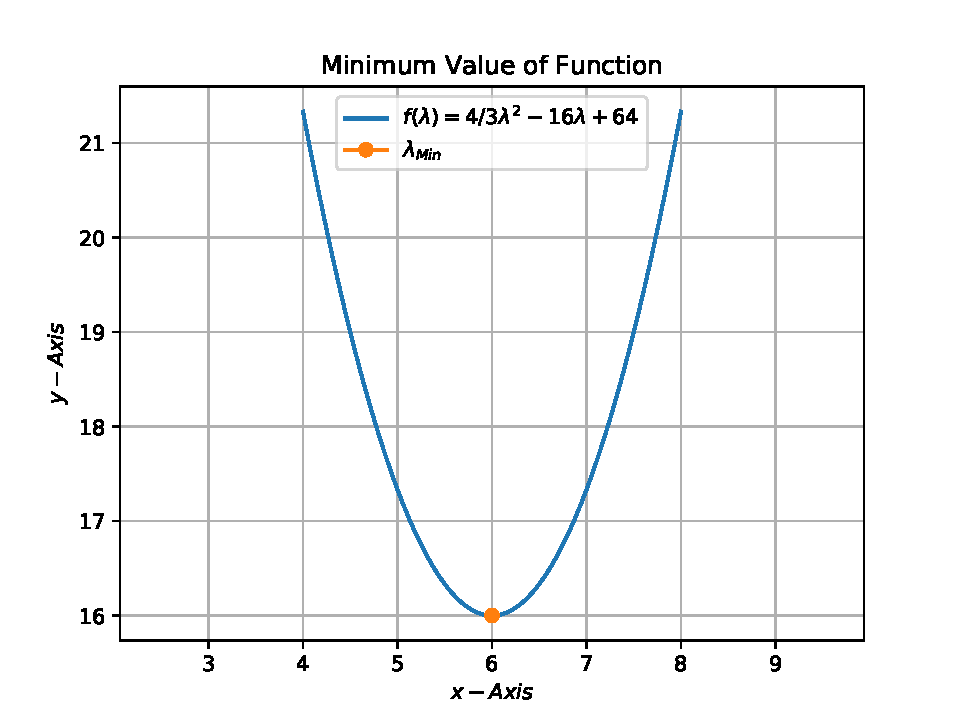
\includegraphics[width=\columnwidth]{11/10/3/3/1/conv/figs/problem3.1a.pdf}
	\end{center}
\caption{}
\label{fig:11/10/3/3/1/conv/Fig1}
\end{figure}
\begin{figure}[!h]
	\begin{center}
		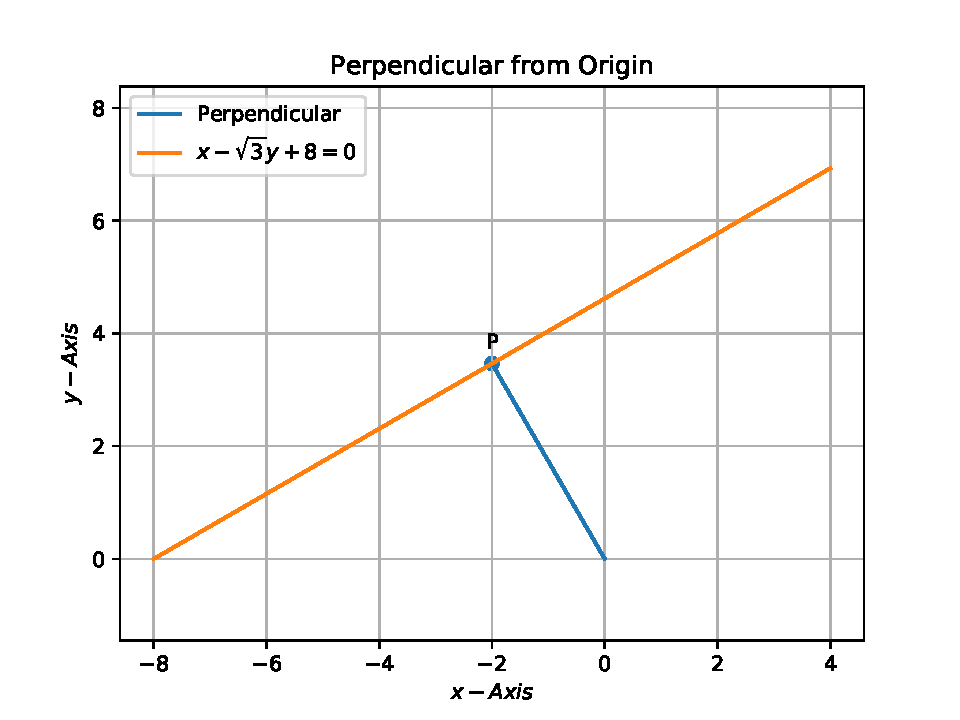
\includegraphics[width=\columnwidth]{11/10/3/3/1/conv/figs/problem3.1b.pdf}
	\end{center}
\caption{}
\label{fig:11/10/3/3/1/conv/Fig2}
\end{figure}

		\item Reduce the equation $y-2=0$ into normal form. Find the perpendicular distances from the origin and angle between perpendicular and the positive x-axis.
			\\
\solution 
\label{11/10/3/3/2/conv}
\iffalse
\documentclass[12pt]{article}
\usepackage{graphicx}
\usepackage{amsmath}
\usepackage{mathtools}
\usepackage{gensymb}
\usepackage{tabularx}
\usepackage{array}
\usepackage[latin1]{inputenc}
\usepackage{fullpage}
\usepackage{color}
\usepackage{array}
\usepackage{longtable}
\usepackage{calc}
\usepackage{multirow}
\usepackage{hhline}
\usepackage{ifthen}
\usepackage{lscape}
\usepackage{float}
\usepackage{amssymb}

\newcommand{\mydet}[1]{\ensuremath{\begin{vmatrix}#1\end{vmatrix}}}
\providecommand{\brak}[1]{\ensuremath{\left(#1\right)}}
\providecommand{\norm}[1]{\left\lVert#1\right\rVert}
\providecommand{\abs}[1]{\left\vert#1\right\vert}
\newcommand{\solution}{\noindent \textbf{Solution: }}
\newcommand{\myvec}[1]{\ensuremath{\begin{pmatrix}#1\end{pmatrix}}}
\let\vec\mathbf

\def\inputGnumericTable{}

\begin{document}
\begin{center}
\textbf\large{OPTIMIZATION}

\end{center}
\section*{Excercise 10.3}


\solution
\fi
The given equation can be written as
\begin{align}
	\label{eq:11/10/3/3/2/conv/eq1}
	\myvec{0&1}\vec{x} &= 2\\
\implies 	\vec{n} &= \myvec{0\\1},\,
	\vec{m} = \myvec{1\\0}
\end{align}
Equation \eqref{eq:11/10/3/3/2/conv/eq1} can be represented in parametric form as
\begin{align}
	\label{eq:11/10/3/3/2/conv/eq2}
	\vec{x} = \vec{A}+\lambda\vec{m}
\end{align}
where
\begin{align}
	\vec{A} &= \myvec{2\\2}.
	\label{eq:11/10/3/3/2/conv/line}
\end{align}
Let $\vec{O}$ be the origin. The perpendicular distance will be the minimum distance from $\vec{O}$ to the line. Let $\vec{P}$ be the foot of perpendicular. This problem can be formulated as an optimization problem as 
\begin{align}
	d &=  \min_{\vec{x}}\norm{\vec{x}-\vec{O}}^2\\
	&=\min_{\lambda}\norm{\vec{A}+\lambda\vec{m}-\vec{O}}^2\\
	&= f\brak{\lambda} = \norm{\vec{m}}^2\lambda^2+2\vec{A}^\top\vec{m}+\norm{\vec{A}}^2
	\label{eq:11/10/3/3/2/conv/eq3}
	\\
	&= \lambda^2+4\lambda+8
\end{align}
$\because$ the coefficient of $\lambda^2>0$, \eqref{eq:11/10/3/3/2/conv/eq3} is convex. 
\begin{align}
	\label{eq:11/10/3/3/2/conv/eq4}
	f^\prime\brak{\lambda} = 2\norm{\vec{m}}^2\lambda+\brak{\vec{A}^\top\vec{m}+\vec{m}^\top\vec{A}}
\end{align}
\begin{enumerate}
\item Computing $\lambda_{min}$ using Derivative method
\begin{align}
	f^{\prime\prime}\brak{\lambda} &= 2\\
	\because f^{\prime\prime}\brak{\lambda}>0,&f^{\prime}\brak{\lambda_{min}}=0, \text{ for } \lambda_{min}\\
	f^{\prime}\brak{\lambda_{min}} &= 2\norm{\vec{m}}^2\lambda_{min}+\brak{\vec{A}^\top\vec{m}+\vec{m}^\top\vec{A}}\\
	\therefore \lambda_{min} &= -\frac{\brak{\vec{A}^\top\vec{m}+\vec{m}^\top\vec{A}}}{2\norm{\vec{m}}^2} = -2
\end{align}
Thus, 
\begin{align}
	\vec{x}_{min} &= \vec{P} = \myvec{2\\2}+\brak{-2}\myvec{1\\0}\\
	&= \myvec{0\\2}\\
	OP &= \norm{\vec{P}-\vec{O}}\\
	&= \norm{\myvec{0\\2}-\myvec{0\\0}}\\
	&= 2
\end{align}
\item Solving using cvxpy, with
\begin{align}
	\vec{n} &= \myvec{0\\1}\\
	\vec{O} &= \myvec{0\\0}\\
	c &= 2\\
	&\min_{\vec{x}}\norm{\vec{x}-\vec{O}}^2 = 2, \vec{x}_{min} = \myvec{0\\2}
\end{align}
\end{enumerate}
See Figs. \ref{fig:11/10/3/3/2/conv/Fig1} and \ref{fig:11/10/3/3/2/conv/Fig2}.
\begin{figure}[!h]
	\begin{center} 
	    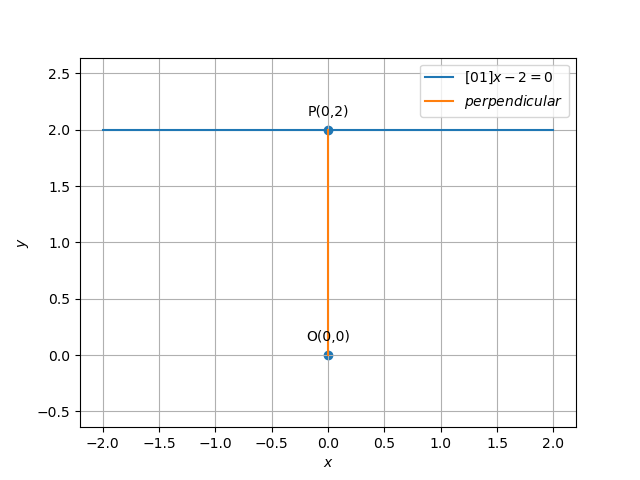
\includegraphics[width=\columnwidth]{11/10/3/3/2/conv/figs/opt1}
	\end{center}
\caption{}
\label{fig:11/10/3/3/2/conv/Fig1}
\end{figure}
\begin{figure}[!h]
	\begin{center} 
	    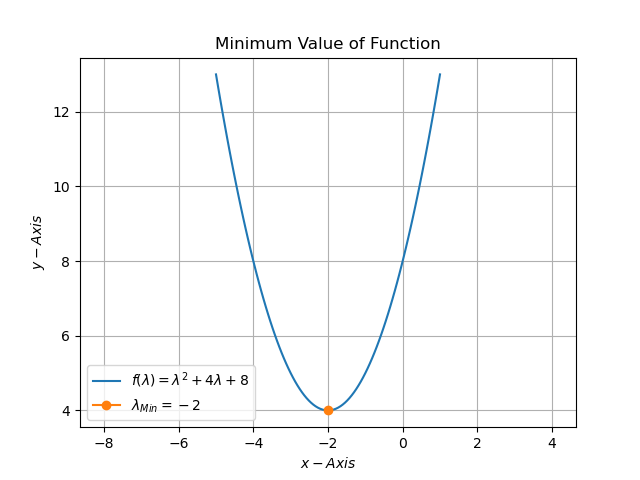
\includegraphics[width=\columnwidth]{11/10/3/3/2/conv/figs/opt2}
	\end{center}
\caption{}
\label{fig:11/10/3/3/2/conv/Fig2}
\end{figure}

 \item Find the coordinates of the foot of perpendicular from the point 
    \begin{align}
        \vec{P} = \myvec{-1\\3}
        \label{eq:11/10/3/14/conv/P-def}
    \end{align}
    to the line 
    \begin{align}
        \myvec{3&-4}\vec{x} = 16
        \label{eq:11/10/3/14/conv/line}
    \end{align}
			\\
\solution 
\label{11/10/3/14/conv}
\iffalse
\documentclass[journal,12pt,twocolumn]{IEEEtran}
\usepackage{setspace}
\usepackage{gensymb}
\singlespacing
\usepackage[cmex10]{amsmath}
\usepackage{amsthm}
\usepackage{mathrsfs}
\usepackage{txfonts}
\usepackage{stfloats}
\usepackage{bm}
\usepackage{cite}
\usepackage{cases}
\usepackage{subfig}
\usepackage{longtable}
\usepackage{multirow}
\usepackage{enumitem}
\usepackage{mathtools}
\usepackage{tikz}
\usepackage{circuitikz}
\usepackage{verbatim}
\usepackage[breaklinks=true]{hyperref}
\usepackage{tkz-euclide} % loads  TikZ and tkz-base
\usepackage{listings}
\usepackage{color}    
\usepackage{array}    
\usepackage{longtable}
\usepackage{calc}     
\usepackage{multirow} 
\usepackage{hhline}   
\usepackage{ifthen}   
\usepackage{lscape}     
\usepackage{chngcntr}
\DeclareMathOperator*{\Res}{Res}
\renewcommand\thesection{\arabic{section}}
\renewcommand\thesubsection{\thesection.\arabic{subsection}}
\renewcommand\thesubsubsection{\thesubsection.\arabic{subsubsection}}

\renewcommand\thesectiondis{\arabic{section}}
\renewcommand\thesubsectiondis{\thesectiondis.\arabic{subsection}}
\renewcommand\thesubsubsectiondis{\thesubsectiondis.\arabic{subsubsection}}
\renewcommand\thetable{\arabic{table}}
% correct bad hyphenation here
\hyphenation{op-tical net-works semi-conduc-tor}
\def\inputGnumericTable{}                                 %%

\lstset{
%language=C,
frame=single, 
breaklines=true,
columns=fullflexible
}
%\lstset{
%language=tex,
%frame=single, 
%breaklines=true
%}

\begin{document}
\newtheorem{theorem}{Theorem}[section]
\newtheorem{problem}{Problem}
\newtheorem{proposition}{Proposition}[section]
\newtheorem{lemma}{Lemma}[section]
\newtheorem{corollary}[theorem]{Corollary}
\newtheorem{example}{Example}[section]
\newtheorem{definition}[problem]{Definition}
\newcommand{\BEQA}{\begin{eqnarray}}
\newcommand{\EEQA}{\end{eqnarray}}
\newcommand{\define}{\stackrel{\triangle}{=}}
\bibliographystyle{IEEEtran}
\providecommand{\mbf}{\mathbf}
\providecommand{\pr}[1]{\ensuremath{\Pr\left(#1\right)}}
\providecommand{\qfunc}[1]{\ensuremath{Q\left(#1\right)}}
\providecommand{\sbrak}[1]{\ensuremath{{}\left[#1\right]}}
\providecommand{\lsbrak}[1]{\ensuremath{{}\left[#1\right.}}
\providecommand{\rsbrak}[1]{\ensuremath{{}\left.#1\right]}}
\providecommand{\brak}[1]{\ensuremath{\left(#1\right)}}
\providecommand{\lbrak}[1]{\ensuremath{\left(#1\right.}}
\providecommand{\rbrak}[1]{\ensuremath{\left.#1\right)}}
\providecommand{\cbrak}[1]{\ensuremath{\left\{#1\right\}}}
\providecommand{\lcbrak}[1]{\ensuremath{\left\{#1\right.}}
\providecommand{\rcbrak}[1]{\ensuremath{\left.#1\right\}}}
\theoremstyle{remark}
\newtheorem{rem}{Remark}
\newcommand{\sgn}{\mathop{\mathrm{sgn}}}
\providecommand{\abs}[1]{\left\vert#1\right\vert}
\providecommand{\res}[1]{\Res\displaylimits_{#1}} 
\providecommand{\norm}[1]{\left\lVert#1\right\rVert}
\providecommand{\mtx}[1]{\mathbf{#1}}
\providecommand{\mean}[1]{E\left[ #1 \right]}
\providecommand{\fourier}{\overset{\mathcal{F}}{ \rightleftharpoons}}
\providecommand{\system}[1]{\overset{\mathcal{#1}}{ \longleftrightarrow}}
\newcommand{\solution}{\noindent \textbf{Solution: }}
\newcommand{\cosec}{\,\text{cosec}\,}
\providecommand{\dec}[2]{\ensuremath{\overset{#1}{\underset{#2}{\gtrless}}}}
\newcommand{\myvec}[1]{\ensuremath{\begin{pmatrix}#1\end{pmatrix}}}
\newcommand{\mydet}[1]{\ensuremath{\begin{vmatrix}#1\end{vmatrix}}}
\let\vec\mathbf
\def\putbox#1#2#3{\makebox[0in][l]{\makebox[#1][l]{}\raisebox{\baselineskip}[0in][0in]{\raisebox{#2}[0in][0in]{#3}}}}
     \def\rightbox#1{\makebox[0in][r]{#1}}
     \def\centbox#1{\makebox[0in]{#1}}
     \def\topbox#1{\raisebox{-\baselineskip}[0in][0in]{#1}}
     \def\midbox#1{\raisebox{-0.5\baselineskip}[0in][0in]{#1}}

\vspace{3cm}
\title{Optimization Assignment}
\author{Gautam Singh}
\maketitle
\bigskip

\begin{abstract}
    This document contains the solution to Question 4 of Exercise 2 in Chapter
    10 of the class 11 NCERT textbook.
\end{abstract}

\begin{enumerate}
   
    \solution 
    \fi
		Any point on \eqref{eq:11/10/3/14/conv/line} is clearly of the form
    \begin{align}
        \vec{Q} = \vec{A} + \lambda\vec{m}
        \label{eq:11/10/3/14/conv/Q-def}
    \end{align}
    where $\lambda \in \mathbb{R}$ and
    \begin{align}
        \vec{A} = \myvec{0\\-4},\ \vec{m} = \myvec{4\\3}
        \label{eq:11/10/3/14/conv/vals}
    \end{align}
    Thus,
    \begin{align}
        f\brak{\lambda} &= \norm{\vec{Q}-\vec{P}}^2 \\
                        &= \norm{\vec{A}-\vec{P}+\lambda\vec{m}}^2 \\
                        &= \norm{\vec{m}}^2\lambda^2 + 2\vec{m}^\top\brak{\vec{A}-\vec{P}}\lambda + \norm{\vec{A}-\vec{P}}^2
                        \label{eq:11/10/3/14/conv/dist-lambda}
    \end{align}
    Since the coefficient of $\lambda^2$ in $f(\lambda)$ is positive, it
    follows that $f\brak{\lambda}$ is convex. Hence, the minima is achieved at
    \begin{align}
        f'\brak{\lambda_m} &= 2\brak{\norm{\vec{m}}^2\lambda_m + \vec{m}^\top\brak{\vec{A}-\vec{P}}} = 0 \\
        \implies \lambda_m &= -\frac{\vec{m}^\top\brak{\vec{A}-\vec{P}}}{\norm{\vec{m}}^2}
        \label{eq:11/10/3/14/conv/lambda-min}
    \end{align}
    Thus,
    \begin{align}
        \vec{Q_m} &= \vec{A} + \lambda_m\vec{m} \\
                  &= \vec{A} - \frac{\vec{m}^\top\brak{\vec{A}-\vec{P}}}{\norm{\vec{m}}^2}\vec{m}
                  \label{eq:11/10/3/14/conv/Q-m-exp}
    \end{align}
    Thus, substituting \eqref{eq:11/10/3/14/conv/vals} into \eqref{eq:11/10/3/14/conv/Q-m-exp}, we get
    \begin{align}
        \vec{Q_m} = \frac{1}{25}\myvec{68\\-49}
        \label{eq:11/10/3/14/conv/Q-sol}
    \end{align}
    The value of $\lambda_m$ is verified in Fig. \ref{fig:11/10/3/14/conv/convex}.
		\begin{figure}[!ht]
        \centering
        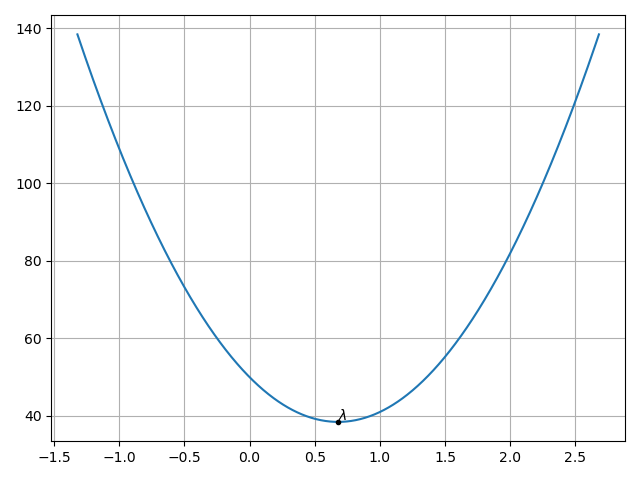
\includegraphics[width=\columnwidth]{11/10/3/14/conv/figs/convex.png}
        \caption{This convex function achieves its minimum at $\lambda_m$.}
        \label{fig:11/10/3/14/conv/convex}
    \end{figure}



	\item Determine if the following are convex functions
\begin{enumerate}
\item Determine whether the function $f\brak{x} = \brak{2x-1}^2 + 3$ is convex or not. \\ 
\solution 
\label{12/6/5/1/1/conv}
%\iffalse
\documentclass[journal,12pt,twocolumn]{IEEEtran}
\usepackage{romannum}
\usepackage{float}
\usepackage{setspace}
\usepackage{gensymb}
\singlespacing
\usepackage[cmex10]{amsmath}
\usepackage{amsthm}
\usepackage{mathrsfs}
\usepackage{txfonts}
\usepackage{stfloats}
\usepackage{bm}
\usepackage{cite}
\usepackage{cases}
\usepackage{subfig}
\usepackage{longtable}
\usepackage{multirow}
\usepackage{enumitem}
\usepackage{mathtools}
\usepackage{steinmetz}
\usepackage{tikz}
\usepackage{circuitikz}
\usepackage{verbatim}
\usepackage{tfrupee}
\usepackage[breaklinks=true]{hyperref}
\usepackage{tkz-euclide}
\usetikzlibrary{calc,math}
\usepackage{listings}
    \usepackage{color}                                            %%
    \usepackage{array}                                            %%
    \usepackage{longtable}                                        %%
    \usepackage{calc}                                             %%
    \usepackage{multirow}                                         %%
    \usepackage{hhline}                                           %%
    \usepackage{ifthen}                                           %%
  %optionally (for landscape tables embedded in another document): %%
    \usepackage{lscape}     
\usepackage{multicol}
\usepackage{chngcntr}
\DeclareMathOperator*{\Res}{Res}
\renewcommand\thesection{\arabic{section}}
\renewcommand\thesubsection{\thesection.\arabic{subsection}}
\renewcommand\thesubsubsection{\thesubsection.\arabic{subsubsection}}

\renewcommand\thesectiondis{\arabic{section}}
\renewcommand\thesubsectiondis{\thesectiondis.\arabic{subsection}}
\renewcommand\thesubsubsectiondis{\thesubsectiondis.\arabic{subsubsection}}

% correct bad hyphenation here
\hyphenation{op-tical net-works semi-conduc-tor}
\def\inputGnumericTable{}                                 %%

\lstset{
frame=single, 
breaklines=true,
columns=fullflexible
}

\begin{document}


\newtheorem{theorem}{Theorem}[section]
\newtheorem{problem}{Problem}
\newtheorem{proposition}{Proposition}[section]
\newtheorem{lemma}{Lemma}[section]
\newtheorem{corollary}[theorem]{Corollary}
\newtheorem{example}{Example}[section]
\newtheorem{definition}[problem]{Definition}
\newcommand{\BEQA}{\begin{eqnarray}}
\newcommand{\EEQA}{\end{eqnarray}}
\newcommand{\define}{\stackrel{\triangle}{=}}

\bibliographystyle{IEEEtran}
\providecommand{\mbf}{\mathbf}
\providecommand{\pr}[1]{\ensuremath{\Pr\left(#1\right)}}
\providecommand{\qfunc}[1]{\ensuremath{Q\left(#1\right)}}
\providecommand{\sbrak}[1]{\ensuremath{{}\left[#1\right]}}
\providecommand{\lsbrak}[1]{\ensuremath{{}\left[#1\right.}}
\providecommand{\rsbrak}[1]{\ensuremath{{}\left.#1\right]}}
\providecommand{\brak}[1]{\ensuremath{\left(#1\right)}}
\providecommand{\lbrak}[1]{\ensuremath{\left(#1\right.}}
\providecommand{\rbrak}[1]{\ensuremath{\left.#1\right)}}
\providecommand{\cbrak}[1]{\ensuremath{\left\{#1\right\}}}
\providecommand{\lcbrak}[1]{\ensuremath{\left\{#1\right.}}
\providecommand{\rcbrak}[1]{\ensuremath{\left.#1\right\}}}
\theoremstyle{remark}
\newtheorem{rem}{Remark}
\newcommand{\sgn}{\mathop{\mathrm{sgn}}}
\providecommand{\abs}[1]{\left\vert#1\right\vert}
\providecommand{\res}[1]{\Res\displaylimits_{#1}} 
\providecommand{\norm}[1]{\left\lVert#1\right\rVert}
\providecommand{\mtx}[1]{\mathbf{#1}}
\providecommand{\mean}[1]{E\left[ #1 \right]}
\providecommand{\fourier}{\overset{\mathcal{F}}{ \rightleftharpoons}}
\providecommand{\system}{\overset{\mathcal{H}}{ \longleftrightarrow}}
\newcommand{\solution}{\noindent \textbf{Solution: }}
\newcommand{\cosec}{\,\text{cosec}\,}
\providecommand{\dec}[2]{\ensuremath{\overset{#1}{\underset{#2}{\gtrless}}}}
\newcommand{\myvec}[1]{\ensuremath{\begin{pmatrix}#1\end{pmatrix}}}
\newcommand{\mydet}[1]{\ensuremath{\begin{vmatrix}#1\end{vmatrix}}}
\numberwithin{equation}{subsection}
\makeatletter
\@addtoreset{figure}{problem}
\makeatother

\let\StandardTheFigure\thefigure
\let\vec\mathbf
\renewcommand{\thefigure}{\theproblem}



\def\putbox#1#2#3{\makebox[0in][l]{\makebox[#1][l]{}\raisebox{\baselineskip}[0in][0in]{\raisebox{#2}[0in][0in]{#3}}}}
     \def\rightbox#1{\makebox[0in][r]{#1}}
     \def\centbox#1{\makebox[0in]{#1}}
     \def\topbox#1{\raisebox{-\baselineskip}[0in][0in]{#1}}
     \def\midbox#1{\raisebox{-0.5\baselineskip}[0in][0in]{#1}}

\vspace{3cm}


\title{Assignment 1}
\author{Jaswanth Chowdary Madala}





% make the title area
\maketitle

\newpage

%\tableofcontents

\bigskip

\renewcommand{\thefigure}{\theenumi}
\renewcommand{\thetable}{\theenumi}

\begin{enumerate}

\textbf{Solution:} 
\fi
		The lines $l_1$ and $l_2$ in vector form can be written as
\begin{align}
\vec{x} &= \myvec{1\\1\\0} + \lambda_1\myvec{2\\-1\\1}\\
\vec{x} &= \myvec{2\\1\\-1} + \lambda_2\myvec{3\\-5\\2}\\
\vec{x_1} = \myvec{1\\1\\0},\, \vec{x_2} &= \myvec{2\\1\\-1}, \,\vec{m_1} = \myvec{2\\-1\\1}, \, \vec{m_2} = \myvec{3\\-5\\2}
\end{align}
The distance between the lines is given by,
\begin{align}
d &= \norm{\brak{\vec{x_2}+ \lambda_2\vec{m_2}} - \brak{\vec{x_1}+ \lambda_1\vec{m_1}}}\\
\implies d &= \norm{\vec{x_2}-\vec{x_1}-\lambda_1\vec{m_1}+\lambda_2\vec{m_2}} \label{eq:12/11/2/e11/conv1}
\end{align}
Consider the following definitions
\begin{align}
\vec{A} &\triangleq \vec{x_2} - \vec{x_1} ,\,
\vec{M} &\triangleq \myvec{\vec{m_1} & \vec{m_2}} ,\,
\bm{\lambda} &\triangleq \myvec{\lambda_1\\-\lambda_2} \label{eq:12/11/2/e11/conv4}
\end{align}
From  \eqref{eq:12/11/2/e11/conv4},
\begin{align}
d = \norm{\vec{A}-\vec{M}\bm{\lambda}}
\end{align}
Here we have the values of $\vec{A}, \vec{M}$ as
\begin{align}
\vec{M} &= \myvec{2&3\\-1&-5\\1&2},\,
\vec{A} &= \myvec{1\\0\\-1}
\end{align}
The given problem can be formulated as 
\begin{align}
\min_{\bm{\lambda}} d^2 &= \bm{\lambda}^{\top}\vec{M}^\top\vec{M}\bm{\lambda} - 2\vec{A}^\top\vec{M}\bm{\lambda}+\vec{A}^\top\vec{A}\\
\text{s.t.} \quad \bm{\lambda} &\in \mathbb{R}^2 
\end{align}
By solving using cvxpy, we get
\begin{align}
\min_{\bm{\lambda}} d &= 1.3019 \\
\bm{\lambda} &= \myvec{0.4237 \\-0.1186} 
\end{align}

The shortest distance between the given lines is $1.3019$ units.

\begin{figure}[!ht]
\centering
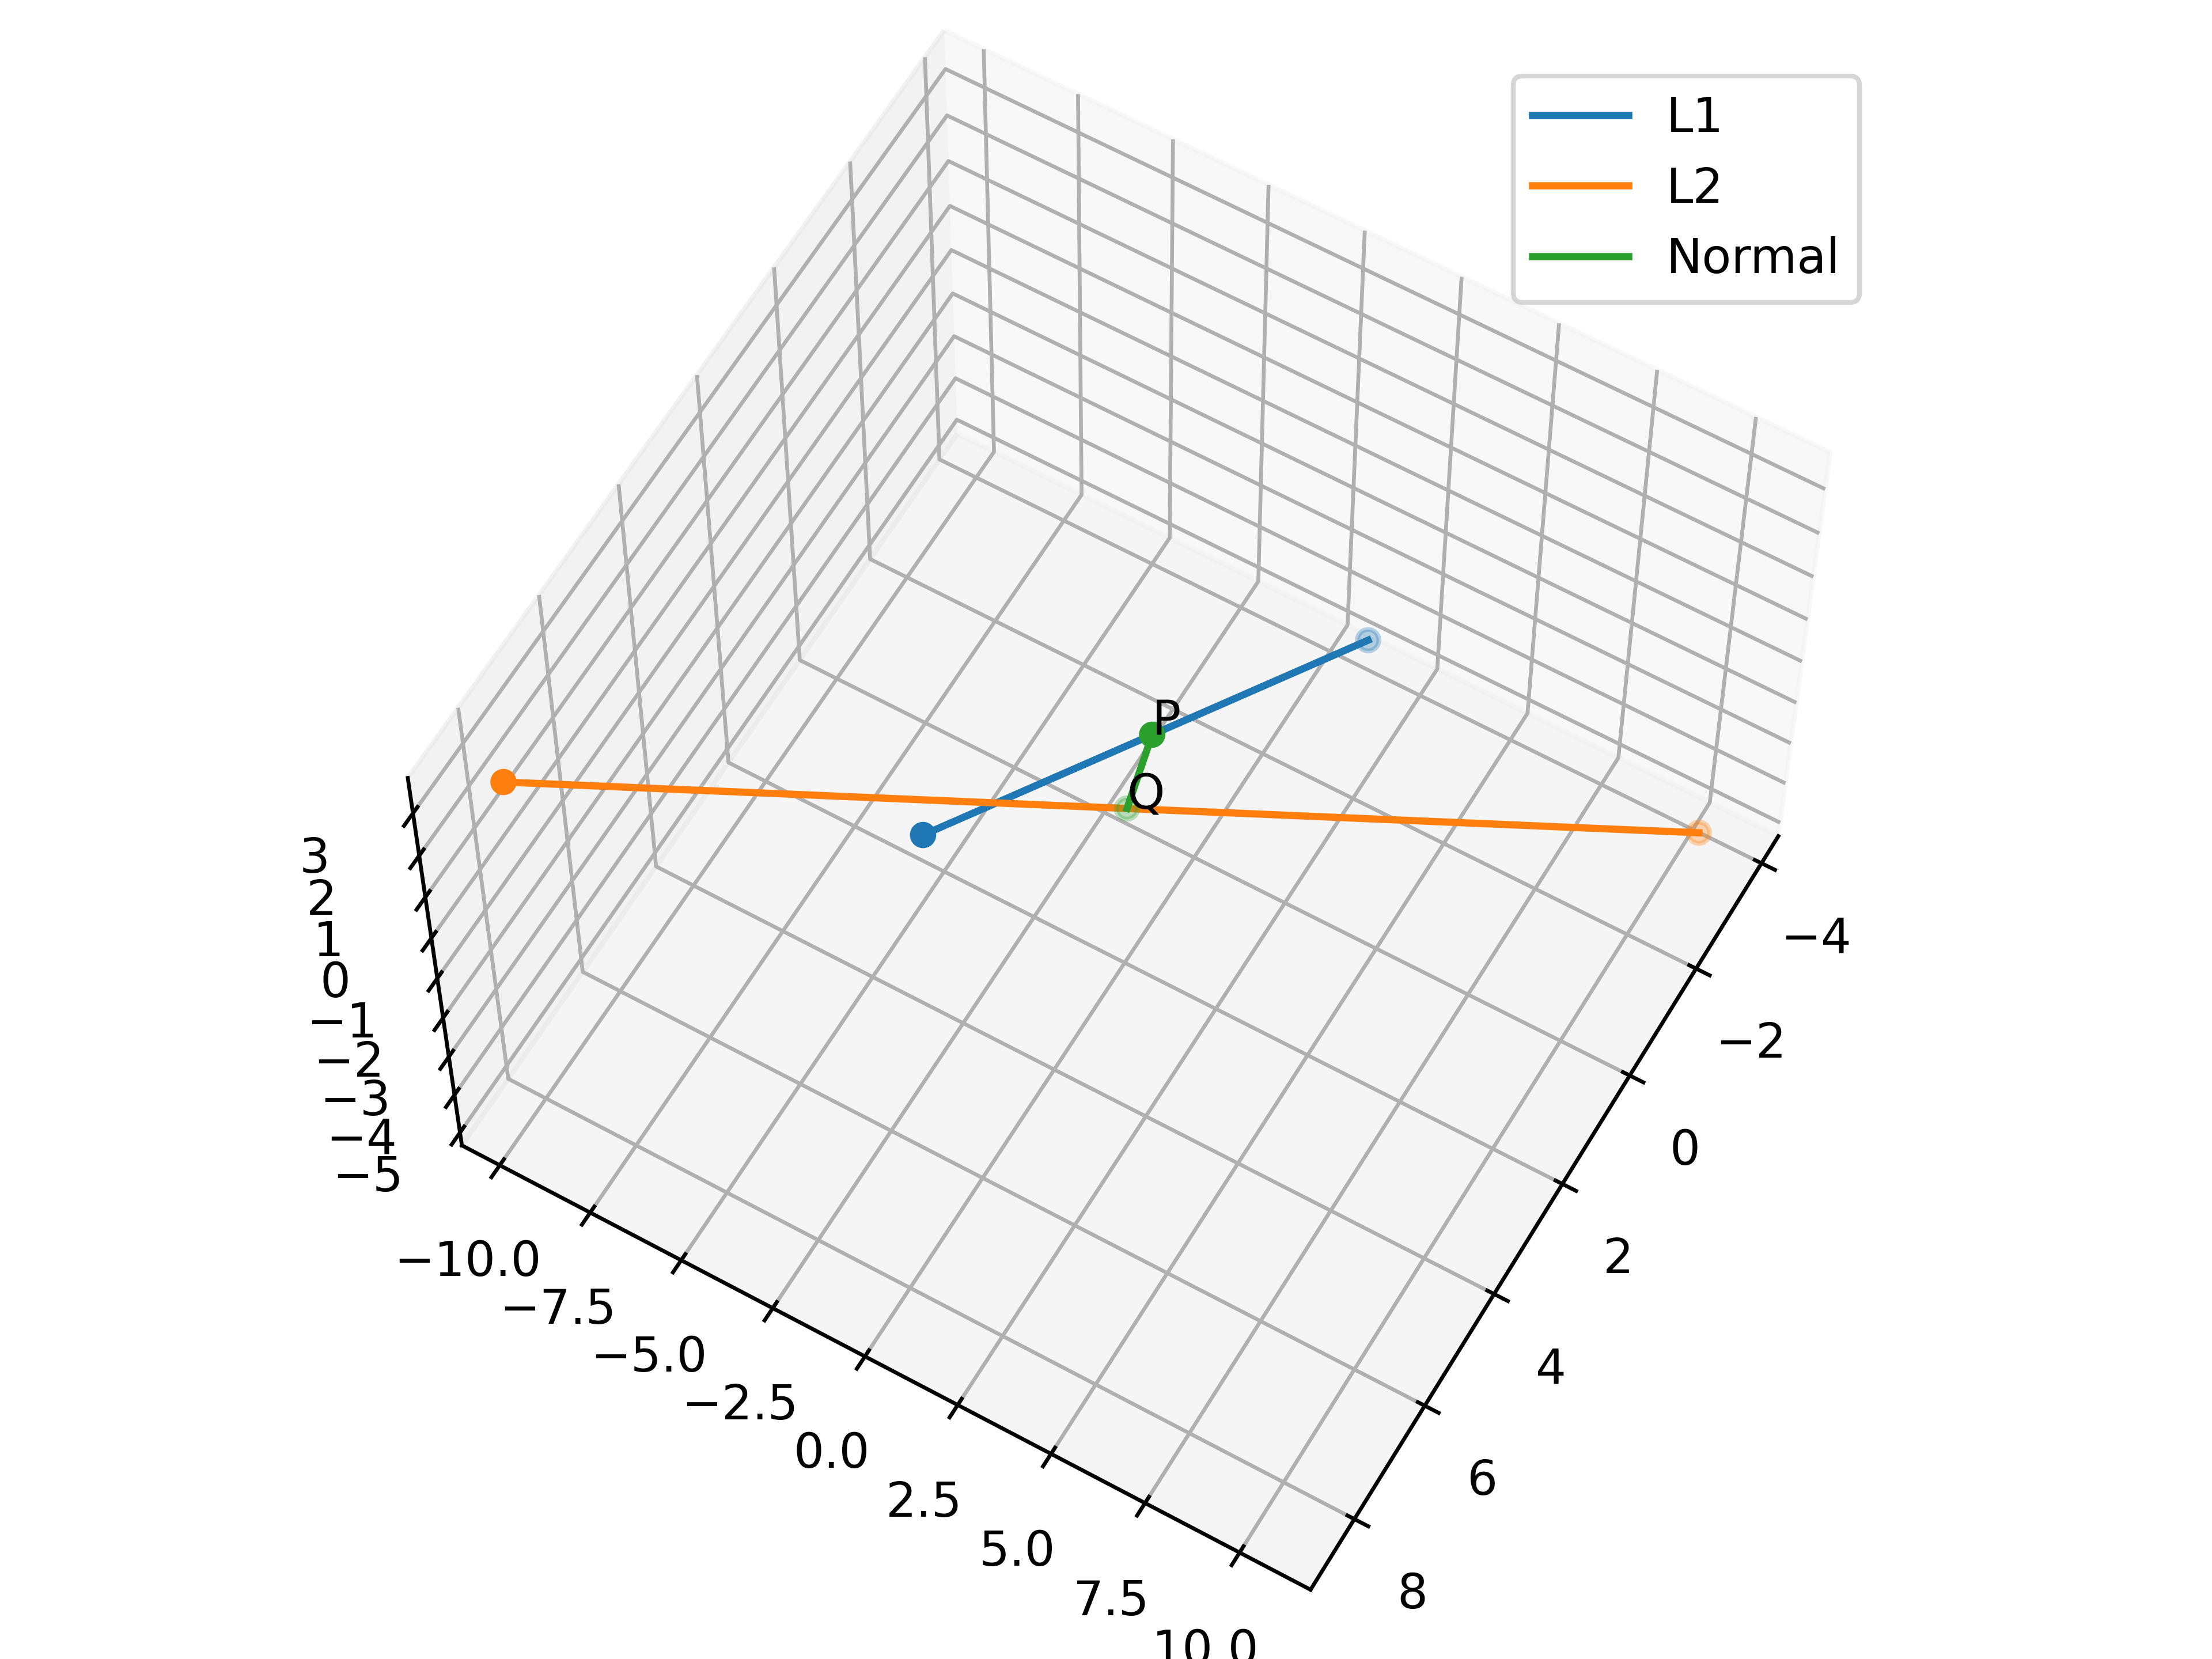
\includegraphics[width=\columnwidth]{12/11/2/e11/conv/figs/skew.png}
\caption{$PQ$ is the required shortest distance.}
	\label{fig:12/11/2/e11/conv}
\end{figure}

	\end{enumerate}
\item
At what points in the interval (0,2$\pi$) does the function $\sin2x$ attain its maximum value.
\label{12/6/5/8/1}
%\iffalse
\documentclass[journal,10pt,twocolumn]{article}
\usepackage{graphicx, float}
\usepackage[margin=0.5in]{geometry}
\usepackage{amsmath, bm}
\usepackage{array}
\usepackage{booktabs}
\usepackage{mathtools}

\providecommand{\norm}[1]{\left\lVert#1\right\rVert}
\let\vec\mathbf
\newcommand{\myvec}[1]{\ensuremath{\begin{pmatrix}#1\end{pmatrix}}}
\newcommand{\mydet}[1]{\ensuremath{\begin{vmatrix}#1\end{vmatrix}}}

\title{\textbf{Optimization Assignment}}
\author{Maddu Dinesh}
\date{September 2022}

\begin{document}

\maketitle
\paragraph{\textit{Problem Statement} -
\fi
At what points in the interval (0,2$\pi$) does the function $\sin2x$ attain its maximum value.
\\
\solution
	\begin{figure}[!ht]
		\centering
		\includegraphics[width=\columnwidth]{12/6/5/8/figs/a.png}
		\caption{}
		\label{fig:12/6/5/8}
  	\end{figure}
\iffalse
\section*{\large Figure}

\begin{figure}[H]
\centering
\includegraphics[width=1\columnwidth]{a.png}
\caption{Graph of f(x)}
\label{fig:triangle}
\end{figure}
\section*{\large Solution}

	
    \subsection*{\normalsize Gradient descent}
\fi    
  Since  
    \begin{align}
	\label{eq:12/6/5/8vol_varx}
	    f(x) &= \sin2x,
	    \\
	    f'(x) &= 2\cos2x
	\end{align}
\iffalse
we have to attain the maximum value of sin2x in the interval [0,2$\pi$]. This can be seen in Figure f(x).
\fi
Using gradient ascent, 
\begin{align}
	x_{n+1} &= x_n + \alpha \nabla f(x_n) \\
&=x_n+\alpha(2\cos2x)
\end{align}
Choosing
\begin{align}
	x_0&=0.5,\alpha=0.001, precision = 0.00000001, 
	\\
	f_{max} &= 1.0000,
 	x_{max}= 0.7854.
    \end{align}
   
    

    





 







\item
Find the absolute maximum and minimum values of the function $f$ given by 
\begin{align}
	f(x) = \cos^2x + \sin x,\quad x \in \sbrak{0,\pi} 
\end{align} 
\label{12/6/6/14/1}
%\iffalse
\documentclass[10pt,twocolumn]{article}
\usepackage{graphicx}
\usepackage[margin=0.5in]{geometry}
\usepackage[cmex10]{amsmath}
\usepackage{array}
\usepackage{booktabs}
\usepackage{mathtools}
\title{\textbf{Optimization Assignment}}
\author{Sinkona Chinthamalla}

\providecommand{\norm}[1]{\lVert#1\rVert}
\providecommand{\abs}[1]{\vert#1\vert}
\let\vec\mathbf
\newcommand{\myvec}[1]{\ensuremath{\begin{pmatrix}#1\end{pmatrix}}}
\newcommand{\mydet}[1]{\ensuremath{\begin{vmatrix}#1\end{vmatrix}}}
\providecommand{\brak}[1]{\ensuremath{\left(#1\right)}}
\providecommand{\lbrak}[1]{\ensuremath{\left(#1\right.}}
\providecommand{\rbrak}[1]{\ensuremath{\left.#1\right)}}
\providecommand{\sbrak}[1]{\ensuremath{{}\left[#1\right]}}

\begin{document}

\maketitle
\paragraph{\textit{Problem Statement} -
\fi
Find the absolute maximum and minimum values of the function $f$ given by 
\begin{align}
	f(x) = \cos^2x + \sin x,\quad x \in \sbrak{0,\pi} 
\end{align} 
\solution
	\begin{figure}[!ht]
		\centering
		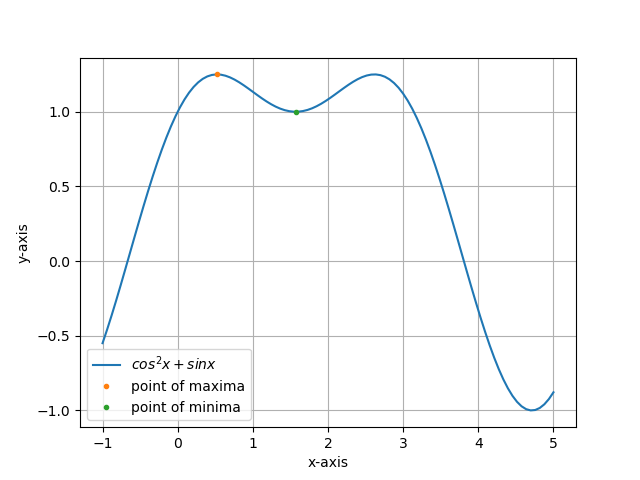
\includegraphics[width=\columnwidth]{12/6/6/14/figs/opt.png}
		\caption{}
		\label{fig:12/6/6/14}
  	\end{figure}
\iffalse

\section{Solution}
\begin{flushleft}
Given function is,\\
\end{flushleft}
\begin{equation}
    f(x)=\cos^2x + \sin x
\end{equation}
\subsection{Calculation using normal differentiation}
\begin{flushleft}
Differentiating (1) yields,
\end{flushleft}
\fi
The derivative of the given function is
\begin{align}
\nabla f(x) = \cos x-2\sin x \cos x 
\end{align}
\iffalse

\noindent Calculating the critical points:
$ \nabla f(x) = 0 $

\begin{equation}
\implies \cos{x} = 0 
\end{equation}
\begin{equation}
\implies -2\sin{x} + 1 = 0
\end{equation}
Therefore, the critical points are 

\begin{equation}
\frac{\pi}{6},\quad\frac{5\pi}{6},\quad\frac{\pi}{2}
\end{equation}

\textbf{1.1.1 Finding absolute maximum and minimum} 
Since given interval is $x \in [0,\pi]$ 

\begin{table}[h]
\centering
\large
\begin{tabular}{|l|l|}
\hline
\textbf{value of x} & \textbf{value of} \\ \hline
At x =0             & 1                 \\ \hline
At x =$ \frac{\pi}{6}$            & $\frac{5}{4}$            \\ \hline
At x =  $ \frac{\pi}{2}$            & 1                 \\ \hline
At x =  $ \frac{5\pi}{6}$            & $\frac{5}{4}$             \\ \hline
at x =       $\pi$       & 1                 \\ \hline
\end{tabular}
\end{table}

Hence, 
\begin{align}
\text{absolute maximum} & =  \frac{5}{4}\\
\text{absolute minimum} & = 1
\end{align}

\subsection{Calculation of Maxima using gradient ascent algorithm}
\fi
The 
maxima is calculated by
\begin{align}
x_{n+1} = x_n + \alpha \nabla f(x_n) 
\\
 &= x_n + \alpha \brak{cosx_n-2sinx_ncosx_n}
\end{align}
where 
\begin{enumerate}
	\item $x_0=0.5$ 
	\item $\alpha=0.001$ 
	\item precision $= 0.00000001$ 
\end{enumerate}
yielding
    \begin{align}
	    f_{max} = 1.25, 
 x_{max}        = 0.52.
    \end{align}
    \iffalse
    
\begin{figure}[h!]
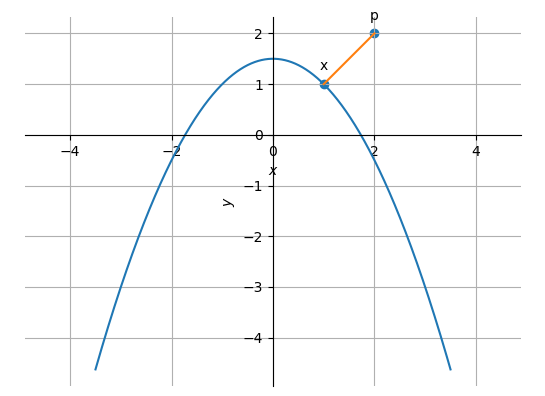
\includegraphics[scale=0.55]{opt.png}
\caption{The function f(x) with maxima and minima points}
\end{figure}        

\subsection{Calculation of Minima using gradient descent algorithm}
To find: 
\begin{align}
\min_{x} f(x)
\end{align}  
Given:
\begin{align}
f(x) = \cos^2x + \sin x,\quad x \in [0,\pi] 
\end{align}
\fi
The 
minima  is found by 
\begin{align}
	x_{n+1} &= x_n - \alpha \nabla f(x_n)
\\
 &= x_n - \alpha \brak{cosx_n-2sinx_ncosx_n}
\end{align}
\iffalse
where \\
1)$x_0=0.5$ \\
2)$\alpha=0.001$ \\
3)precision $= 0.00000001$ \\
values obtained using python are:
    \begin{align}
        \boxed{\text{Minima} = 1 }\\
        \boxed{\text{Minima Point} = 1.57}
    \end{align}

\end{document}
\fi


\end{enumerate}
